



 Suppose $ABCD$ and $CFGH$ are rectangles.  
 \begin{center}
 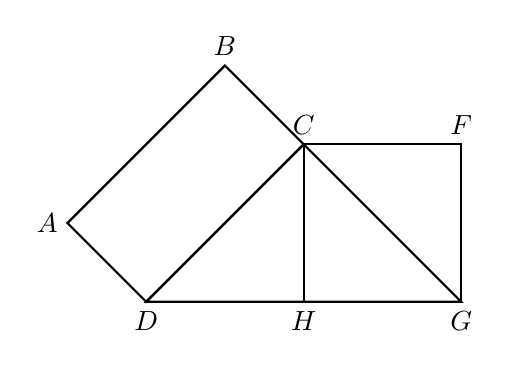
\begin{tikzpicture}
 
 \draw (0,0) --(2,2)--(4,0)--cycle  [thick,-,>=latex];
 \draw (0,0) --(2,2)--(1,3)--(-1,1)--cycle  [thick,-,>=latex];
 \draw (2,0) --(2,2)--(4,2)--(4,0)--cycle  [thick,-,>=latex];
 \draw node[above] at (1,3) {$B$}; 
 \draw node[left] at (-1,1) {$A$};
 \draw node[below] at (0,0) {$D$};
 \draw node[above] at (4,2) {$F$};
 \draw node[below] at (4,0) {$G$};
 \draw node[below] at (2,0) {$H$};
 \draw node[above] at (2,2) {$C$};   
  
   
  
 
   
\end{tikzpicture}
\end{center}



Which of the following must be true?


\ifsat
	\begin{enumerate}[label=\Alph*)]
		\item    $m\angle CDH=m\angle FCG$
		\item    $m\angle CDH=m\angle CGH$  
		\item $m\angle DCH= m\angle HCG$
		\item  $m\angle CDH=m\angle CGF$ %
	\end{enumerate}
\else
\fi

\ifacteven
	\begin{enumerate}[label=\textbf{\Alph*.},itemsep=\fill,align=left]
		\setcounter{enumii}{5}
		\item    $m\angle CDH=m\angle FCG$
		\item    $m\angle CDH=m\angle CGH$  
		\item $m\angle DCH= m\angle HCG$
		\addtocounter{enumii}{1}
		\item  $m\angle CDH=m\angle CGF$ %
		\item  None of the above
	\end{enumerate}
\else
\fi

\ifactodd
	\begin{enumerate}[label=\textbf{\Alph*.},itemsep=\fill,align=left]
		\item    $m\angle CDH=m\angle FCG$
		\item    $m\angle CDH=m\angle CGH$  
		\item $m\angle DCH= m\angle HCG$
		\item  $m\angle CDH=m\angle CGF$ %
		\item  None of the above
	\end{enumerate}
\else
\fi

\ifgridin
  $m\angle CDH=m\angle CGF$ %

\else
\fi

